%\documentclass[tikz, border=5pt]{standalone}
\begin{document}
	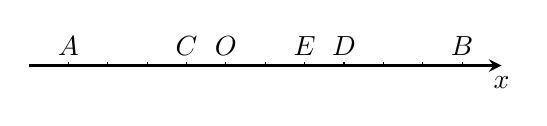
\begin{tikzpicture}[scale=0.5]
		% 绘制带箭头的 x 轴
		\draw[->, >=stealth, line width=1pt] (-5,0) -- (7,0) node[below] {$x$};
		
		% 定义各点坐标(可根据刻度密度调整)
		\coordinate (C) at (-1,0);  % 点 C
		\coordinate (B) at (6,0);  % 点 B
		\coordinate (O) at (0,0);   % 原点 O
		\coordinate (A) at (-4,0);   % 点 A
		\coordinate (D) at (3,0);  % 点 D
		\coordinate (E) at (2,0);  % 点 E

		% 绘制所有小刻度线(从 -5 到 6,每隔 1 单位画竖线)
		\foreach \x in {-4,-3,...,6} {
			\draw (\x, 0.1) -- (\x, 0);  % 小竖线(长 0.1 单位)
		}
		
		% 标记各点标签(位置与原图匹配)
		\node[above] at (C) {$C$};
		\node[above] at (B) {$B$};
		\node[above] at (O) {$O$};
		\node[above] at (A) {$A$};
		\node[above] at (D) {$D$};
		\node[above] at (E) {$E$};
		
	\end{tikzpicture}
\end{document}
